\documentclass{article}

\usepackage{polski}
\usepackage[utf8]{inputenc}
\usepackage{graphicx}
\usepackage{xcolor}
\usepackage{float}
\usepackage{caption}
\usepackage{array}
\usepackage{pbox}

\newcommand\tab[1][1cm]{\hspace*{#1}}

\title{Dokumentacja projektowa}
\date{2018-03-18}
\author{Jędrzej Kozal}

\begin{document}

\begin{titlepage}
	\centering
	
\includegraphics[width=0.25\textwidth]{logo_pol_wroclaw.png}\par\vspace{1cm}
	{\scshape\LARGE Politechnika Wrocławska \par}
	\vspace{1cm}
	{\scshape\Large Miekkie metody obliczeniowe\par}
	\vspace{1.5cm}
	{\huge\bfseries Zastosowanie Sieci Bayesa do diagnozowania ostrych stanów zapalnych \par}
	\vspace{2cm}
	{\Large\itshape Filip Guzy\par}
	{\Large\itshape Jędrzej Kozal\par}
	{\Large\itshape Michał Leś\par}

	\vfill
	prowadzący\par
	Mgr inż.~Mariusz \textsc{Kozioł}

	\vfill

% Bottom of the page
	{\large \today\par}
\end{titlepage}

\tableofcontents
\newpage


\section{Wstęp}

Celem projektu jest zbadanie skuczteczności Sieci Bayesa w automatycznej diagnozie ostrych stanów zapalnych. Określając zagadnienie diagnozowania jako problem klasyfikacji można zmierzyć dokładność uzyskanego modelu. W projekcie wykorzystano sieci QMR i zmierzono dokładność zgodnie z przyjętą metodyką.

\subsection{Wymagania projektowe}
W ramach projektu przewiduje się realizację poniższych podpunktów:
\begin{enumerate}
	\item Analiza danych wejściowych
	\item Przygotowanie danych wejściowych - dychotomizacja, dyskretyzacja
	\item Podział danych wejściowych umożliwiający ocenę klasyfikatora - projekt eksperymentu
	\item Wyznacznie parametrów analizowanego zbioru potrzebnych do skontruowania modelu (określenie prawdopodobieństw a priori i wspólnych rozkładów prawdopodobieństwa)
	\item Przygotowanie modelu - Sieci Bayesa w konfiguracji QMR - wyznazczenie topologii sieci
	\item Weryfikacja skuteczności modelu oraz analiza uzyskanych wyników
\end{enumerate}

Zakłada się, że uzyskany klasyfikator nie będzie klasyfikatorem słabym (klasyfikatory słabe osiągają dokładność zbliżoną do losowego wyboru klasy). Ze względu na brak wiedzy eksperckiej w omawianej dziedzinie, parametry modelu będą określane na podstawie zbioru uczącego. W efekcie powodzenie projektu może być ściśle powiązane z jakością wykorzystanego zbioru danych. 

\subsection{Wykorzystane narzędzia}
Do realizacji zadania wykorzystano środowisko Matlab, wraz z toolboxem BayesNet. Jest to darmowe narzędzie, dostępne do zanstalowania w środowisku Matlab. 

\section{Podstawy teoretyczne}
W tej sekcji zostaną omówione teoretyczne aspekty problemu oraz przyjętych rozwiązań.

\subsection{Omówienie zagadanienia}
W poniżej sekcji przedstawiono medyczne aspekty omawianego problemu.

\subsubsection{Zbiór uczący}
Jako zbiór danych uczących wykorzystano zbiór Acute Inflammations Data Set dostępny w bazie UCI \cite{data set}. Zawiera 120 próbek w większości binarnych lub dyskrenych. Autorzy uworzyli go z myślą o wspieraniu systemu ekspertowego, umożliwiającego diagnozę dwóch chorób układu moczowego - ostrego zapalenia pęcherza moczowego oraz odmiedniczkowego zapalenia nerek. Poniższe charakterystyki chorób zostały zaczerpnięte z opisu zbioru.

\paragraph{Ostre zapalenie pęcherza moczowego}
"Acute inflammation of urinary bladder is
characterised by sudden occurrence of pains in the abdomen region and 
the urination in form of constant urine pushing, micturition pains and 
sometimes lack of urine keeping. Temperature of the body is rising, 
however most often not above 38C. The excreted urine is turbid and 
sometimes bloody. At proper treatment, symptoms decay usually within 
several days. However, there is inclination to returns. At persons with 
acute inflammation of urinary bladder, we should expect that the illness 
will turn into protracted form."

\paragraph{Odmiedniczkowe zapalenie nerek}
"Acute nephritis of renal pelvis origin occurs considerably more often at 
women than at men. It begins with sudden fever, which reaches, and 
sometimes exceeds 40C. The fever is accompanied by shivers and one- or 
both-side lumbar pains, which are sometimes very strong. Symptoms of 
acute inflammation of urinary bladder appear very often. Quite not 
infrequently there are nausea and vomiting and spread pains of whole 
abdomen."

\subsubsection{Lista cech dostępnych w zbiorze uczącym}

W omawianym zbiorze dla każdego pacjenta znajdują się następujące parametry:

\begin{enumerate}
	\item Temperatura pacjenta 35C-42C
	\item Występowanie of nudności tak, nie
	\item Ból lędźwiowy tak, nie
	\item Urine pushing (nieustająca potrzeba oddawania moczu) tak, nie
	\item Ból w trakcie oddawania moczu tak, nie
	\item Pieczenie cewki moczowej, swędzenie, obrzęk ujścia cewki moczowej tak, nie
	\item decyzja: Zapalenie pęcherza moczowego tak, nie
	\item decyzja: Odmiedniczkowe zapalenie nerek tak, nie
\end{enumerate}


\subsection{Sieci Bayesa}

\subsubsection{Modelowanie probabilitystyczne}
W przypadku modelowania zależności między zmiennymi losowymi stosuje się wspólny rozkład prawdopodobieństwa (joint probabilty distribution, jpd). Dla dyskretnych zmiennych losowych stanowi ono tabelę z wszystkimi możliwymi kombinacjami wartości zmiennych. Dla 4 binarnych zmiennych losowych $A, B, C, D$ istnieje $2^4-1 = 15$ elementów tabeli. W ogólności liczba prawdopodobieństw $n$ zmiennych losowych w tabeli wynosi: $2^n - 1$. Funkcje wykładnicze bardzo szybko osiągają duże wartości, przez co modelowanie dla dużego $n$, może stanowić wyzwanie przez dużą liczbę paramterów.

\subsubsection{Definicja sieci Bayesa}
Sieć Bayesa to klasa modeli graficznych, w których do modelowania zależności między zmiennymi losowymi wykorzystuje się acykliczny graf skierowany. Wierzchołki grafu zawierają zmienne losowe, a krawędzie modelują zależności między zmiennymi losowymi. Wierzchołki połączone z wybranym wierzchołkiem przez krawedź wchodzącą nazywamy rodzicami (parent). Wierzchołki połączone przez krawędź wychodzącą nazywamy dziećmi (child). Wierzchołek nie posiadający rodziców nazywany jest korzeniem (root). Krawędzie grafu i jego struktura modelują zależności między zmiennymi losowymi, co pozwala na ogarniczenie ilości parametrów modelu.

\begin{figure}
\centering
	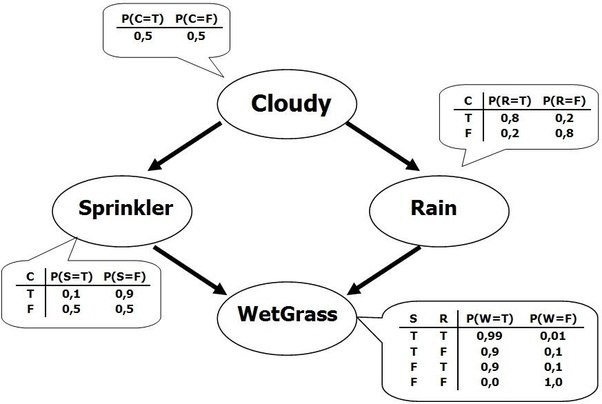
\includegraphics[width=0.80\textwidth]{net.jpeg}\par\vspace{1cm}
\caption{Przykładowa sieć Bayesa, modelująca wilgotność trawy, wraz z lokalnymi wspólnymi rozkładami prawdopodobieństwa. \\ źródło: https://towardsdatascience.com/introduction-to-bayesian-networks-81031eeed94e}
	\label{fig:net}
\end{figure}

Sieć Bayesa wykorzystuje założenie o niezależności zmiennych losowych do obliczania prawdopodobieństwa zmiennych losowych w wezłach, korzystając z prawdopodobieństwa wystąpienia konretnych wartości rodziców. 

Stosując regułę łańcucha dla prawdopodobieństwa, można zapisać wspólny rozkład prawdopodobieństwa jako:

\begin{equation}
	P(A, B, C, D) = P(A|B, C, D)P(B|C, D)P(C|D)P(D)
\end{equation}

Stosując założenie o niezależności $B$ od $C$ i $C$ od $D$ można tą samą regułę uprościć:

\begin{equation}
	P(A, B, C, D) = P(A|B, C, D)P(B|D)P(C)P(D)
\end{equation}

W ogólności dla Sieci Bayesa można zapisać:

\begin{equation}
	P(X_1, ... , X_n) = \prod_{i=1}^{n} P(X_i|Parents(X_i))
\end{equation}

Powoduje to znaczącą redukcję liczby parametrów modelu.

Przykładowa sieć Bayesa wraz z lokalnymi rozkładami prawdopodobieństwa została przedstawiona na rys. \ref{fig:net}. Poprzez podział tabel ze wspólnym rozkładem prawdopodobieństwa na mniejsze ilość paramterów modelu uległa zmianie z 15 do 18. Przy rosnącej ilości parametrów sieci Bayesa mogą przyczynić się do znaczącej redukcji liczby parametrów.

\subsubsection{D-separacja}

Pojęcie D-separacji może zostać wykorzystane do modelowania niezależności danych uczących ze zbioru. Jest ono ściśle powiązane ze strukturą sieci i opiera się na kilku zasadach. Przyjmijmy, że analizujemy dwie zmienne $X$ i $Y$. Zmienna losowa $Z$ znajduje się na ściężce $p$ w grafie między $X$ a $Y$.
\begin{enumerate}
\item Kiedy zmienna losowa $Z$ jest zdarzeniem warunkującym obliczanego prawdopodobieństwa (stanowi dowód, evidence) mówimy, że:
\begin{itemize}
 \item $Z$ jest zablokowane, jeżeli $p$ wchodzi do $Z$ od jego dziecka.
 \item $Z$ jest zablokowane, jeżeli $p$ wchodzi do $Z$ od jego rodzica i wychodzi od jego dziecka.
 \item $Z$ nie jest zablokowane, jeżeli $p$ wchodzi do $Z$ od jego rodzica wychodzi od jego rodzica.
\end{itemize}
\item Kiedy zmienna losowa $Z$ nie jest zdarzeniem warunkującym obliczanego prawdopodobieństwa mówimy, że:
\begin{itemize}
 \item $Z$ nie jest zablokowane, jeżeli $p$ wchodzi do $Z$ od jego dziecka.
 \item $Z$ nie jest zablokowane, jeżeli $p$ wchodzi do $Z$ od jego rodzica i wychodzi od jego dziecka.
 \item $Z$ jest zablokowane, jeżeli $p$ wchodzi do $Z$ od jego rodzica wychodzi od jego rodzica.
\end{itemize}
\end{enumerate}

$X$ jest niezależne od $Y$, jeżeli wszystkie możliwe ścieżki między $X$ a $Y$ w grafie są zablokowane.

$Z$ d-separuje $X$ od $Y$ (zapisywane: $X \perp_G Y|Z$), jeżeli wszystkie ścieżki między $X$ a $Y$ są zablokowane przez $Z$.

\subsubsection{Detekcja topologi sieci na podstawie danych uczących}

Ze względu na brak wiedzy dziedzinowej z zakresu medycyny, oraz braku możliwości konsultacji z ekspertem postanowiono wykorzystać metody pozwalające na nauczenie struktury sieci na podstawie zbioru uczącego.

W \cite{PhD} podano metody uczenia struktury sieci Bayesa. Wyróżna się dwie główne metody. Pierwsza z nich opiera się na maksymalizacji funkcji celu z wykorzystaniem maximum likelihood. Zaproponowano podejście w którym topologia sieci jest modyfikowana zgodnie z kierunkiem wzrostu maximum likelihood (hill climbing).

Drugą metodą opiera się na określeniu topologi na podstawie niezależności zmiennych losowych zbioru uczącego. Skierowany graf acykliczny jest nazywany I-mapą, jeśli:

\begin{equation}
	\forall_{X, Y, Z} (X \perp_G Y| Z) 	\Rightarrow  (X \perp_P Y | Z)
\end{equation}

Korzystając z zależności logicznej:

\begin{equation}
	p \Rightarrow q \Leftrightarrow \neg q \Rightarrow \neg p
\end{equation}

Aplikując poważyszy wzór dla sieci Bayesa można określić, że jeśli w domenowej dystrybucji P zmienne nie są niezależne to również nie powinny być niezależne w grafie (nie są d-separowane). W \cite{PhD} przedstawiono dokładny algorytm określania topologii sieci.

\section{Wykonane eksperymenty}

\section{Uzyskane rezultaty}

\newpage
\begin{thebibliography}{9}

\bibitem{data set}
J.Czerniak, H.Zarzycki, Application of rough sets in the presumptive diagnosis of urinary system diseases, 
Artifical Inteligence and Security in Computing Systems, ACS'2002 9th International Conference Proceedings, 
Kluwer Academic Publishers,2003, pp. 41-51 
\\\texttt{https://archive.ics.uci.edu/ml/datasets/Acute+Inflammations}

\bibitem{paper}
Ben-Gal I., Bayesian Networks, in Ruggeri F., Faltin F. \& Kenett R.,
Encyclopedia of Statistics in Quality \& Reliability, Wiley \& Sons (2007). 
\\\texttt{http://www.eng.tau.ac.il/~bengal/BN.pdf}

\bibitem{PhD}
Learning Bayesian Network Model Structure from Data, Dimitris Margaritis
May 2003, Carnegie Mellon University
\\\texttt{https://www.cs.cmu.edu/~dmarg/Papers/PhD-Thesis-Margaritis.pdf}

\bibitem{Towards Data Sience}
Introduction to Bayesian Networks, Towards Data Sience blog
\\\texttt{https://towardsdatascience.com/introduction-to-bayesian-networks-81031eeed94e}

\bibitem{bayesserver}
Baysian network software for Artificial Inteligence
\\\texttt{https://www.bayesserver.com/docs/introduction/bayesian-networks}

\end{thebibliography}
\newpage

\listoffigures
\newpage

\end{document}